%!TEX root = ../main.tex


\section{Group-based Acceleration}

As discussed above, we can observe that in Section~\ref{subsec:one}, even with the most efficient imputation-in-the-loop  strategy, \ie  one tuple in  each iteration, the time complexity is  $O(KhnL^2)$, where $K$ is the size of the coreset, $h$ is the sample size, $L$ is a small constant and $n$ is the number of entire dataset. Therefore, obviously, the efficiency is dominated by $n$, which is still low when $n$ is large, and thus it  is necessary to further accelerate this process.

\noindent \textbf{Key observation.}   Recap that in Figure~\ref{fig:overviewSingle}, we can observe that  given a tuple $c$ in the coreset, the tuples in the origin full train set $\trainc$ represented by $c$ are likely to be  closer to each other than other tuples not represented by $c$.
Based on this observation, we propose to first cluster the full train set into groups, and then compute the coreset based on these groups. This can achieve much acceleration because the number of groups is much smaller than $n$. 

At the following, we will theoretically and empirically show the groups-based solution can accelerate the coreset selection process without sacrificing the effectiveness much.

%the acceleration can be achieved by clustering the 

\subsection{Group-based Solution Overview}

\begin{figure}[t]
    \centering
    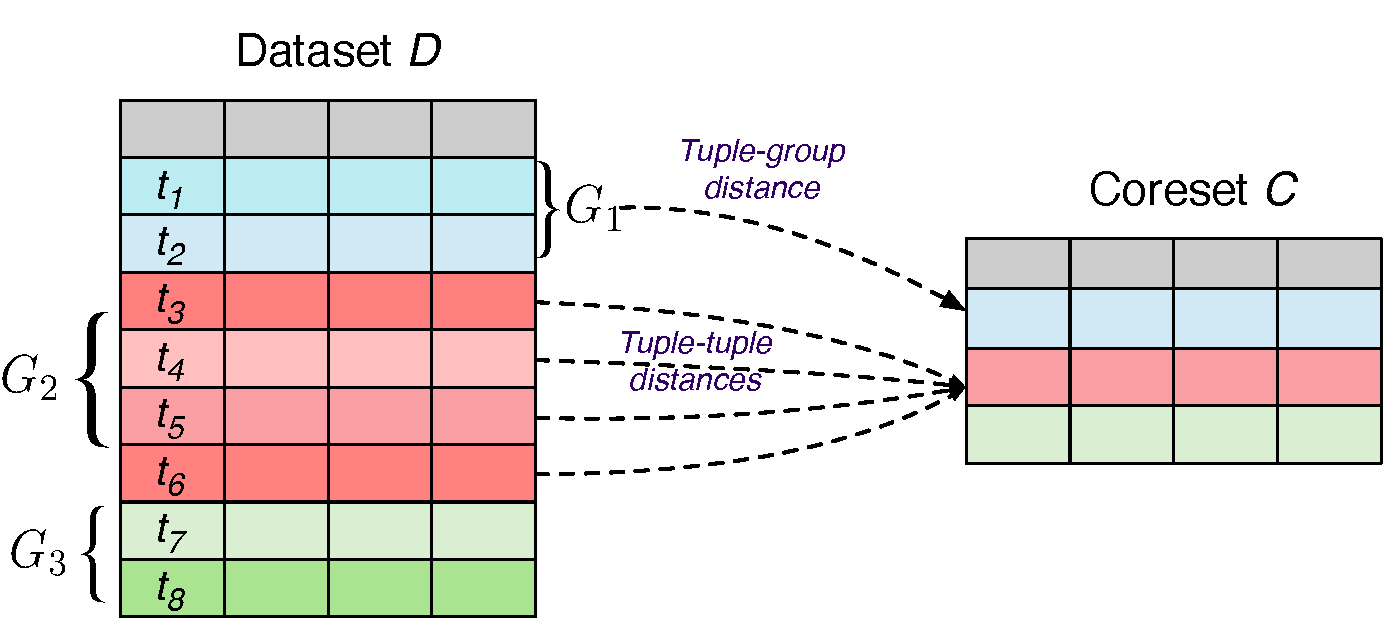
\includegraphics[width=0.6\textwidth]{figs/Overview-gb}
   % \vspace{-2.5em}
    \caption{Illustration of the Group-based Solution.}
    \label{fig:overview-gb}
   % \vspace{-1.5em}
\end{figure}

As shown in Figure~\ref{overview-gb}, one of the core parts of coreset computation is to compute the tuple-tuple distance, \ie $s_{ij}$. For the group-based solution, we just need to consider the relationship between tuples and these pre-computed groups, namely tuple-group distance, rather than the large amount of tuple-tuple distances. As we will discuss below, the computation of tuple-group distance does not need to iterate all tuples in the group, and thus  the overall efficiency can be much improved. 

At a high level, the overall process of group-based \ours solution with imputation in the loop is shown in Algorithm~\ref{alg:group}. To be more explicit, we illustrate Algorithm~\ref{alg:group} in comparison with Algorithm~\ref{alg:framework} in Section~\ref{subsec:framework} without clustering (the modified parts are highlighted in blue fonts).

To be specific, as shown in Line~\ref{alg4:cluster}, we first cluster $\trainc$ into groups using the efficient local sensitive hash (LSH) approach, where each group $\group_u, u\in[1, \groups]$ denotes the indexes of tuples in $\trainc$. In this way, every pair of tuples in the same group is close to each other in the feature distance.
%
 Afterwards, the major difference between group-based \ours and original \ours lies in the 3rd loop. Instead of  selecting a coreset to represent all tuples in the train set, group-based \ours selects a coreset to represent all clusters. As these clusters can well capture the train set distribution, the selected coreset contains enough information to approximate the full gradient of $\trainc$. 
 
 To this end, recap that the typical coreset selection algorithm needs the tuple-tuple distances to approximate the full gradient, while in group-based \ours, we just need to consider the tuple-group distances, \ie  
$\overline{s}_{\gamma(j)k} = \max\limits_{v \in \group_u} s_{\gamma(j)v}, s_{\gamma(j)v} = \lVert\mathbf{x}_v - \mathbf{x}_{\gamma(j)}\rVert, \gamma(j)\in[1, n]$, which denotes the maximum feature distance between the tuple $c_j$ in the coreset and all tuples in $\group_u$. As tuples in $\group_u$ are close to each other, $\overline{s}_{\gamma(j)k}$ can represent the relationship between $c_j$ and tuples in $\group_u$ to a large extent. But as shown in Line~\ref{alg4:bound}, we finally use an upper bound $\bound_{jk}$ to compute the coreset score because computing $\overline{s}_{\gamma(j)k}$ needs to iterate the tuples in $\group_u$, which is time-consuming. Next, we will theoretically show that using the upper bound can still derive a bounded GA error, leading to a well-performed coreset. 

%!TEX root = ../main.tex

\begin{figure}[!t]
 \vspace{-1em}
	\begin{algorithm}[H]
		\normalem
	\caption{Group-based \ours Solution (imputation-in-the-loop) \label{alg:group}}
		{\small
			
		\KwIn{Incomplete train data $\train$, coreset size $\numcore$, sample size $h$.}
		
		\KwOut{A coreset $\core \subseteq \train$, weight $\weightset=\{w_j\}$,$|\core|=|\weightset|=\numcore$.}
		
		$C=\emptyset$;\\\nllabel{alg1:init1}
		
		\add{Cluster $\train$ into groups $\groups = \{ \group_1, \group_2, ..., \group_\groupsize \}$;}\\\nllabel{alg4:cluster}
		
		\While{$|\core|< \numcore$}
		{\nllabel{craig1:loop1}
			
		/*1st loop*/  \\
		
		Sample $h$ tuples as $T_{sample} \subseteq \train \setminus \core$\\\nllabel{craig1:sample}
		
			\For{each tuple $t \in T_{sample}$}  
			{\nllabel{craig1:loop2}
				
				/*2nd loop*/ \\
				 $\hat{\core} = \core \cup \{t\}$;\\
			%	}
			 %$\mathrm{E}[t|\core]=\texttt{ComputeUtility}(t, C,D)$;
				 %/*3rd loop*/  \\\nllabel{craig1:loop3}
				 \For{\add{each group $G_k \in \groups$}}  
				 {
				 	\add{/*3rd loop*/} \\
				 
				 	%	Get the possible worlds of $\hat{\core} \cup \{t_i\}$;\\\nllabel{one:enumw}
				 	%	Compute $\mathrm{E}[\min_{c_j\in \hat{\core}}s_{ij}]$ using these possible worlds and their probabilities;\\\nllabel{one:exp4pw}
				 		\add{$\mathrm{E}[\hat{\core}] +\!\!= \mathrm{E}[\min_{c_j\in \hat{\core}}\bound_{jk} \times |\group_k|]$, where $\bound_{jk}$ is the upper bound of} \\\quad \\\nllabel{alg4:bound} \add{$\overline{s}_{\gamma(j)k} = \max\limits_{v \in \group_k} s_{\gamma(j)v}, s_{\gamma(j)v} = \lVert\mathbf{x}_v - \mathbf{x}_{\gamma(j)}\rVert, \gamma(j)\in[1, n]$; }\\\nllabel{one:dirtysum}
			     }
		         \add{$\mathrm{E}[t|\core] = \mathrm{E}[\core] - \mathrm{E}[\hat{\core}];$}
				 
			}		

			$t^*$ = $\argmax_{t\in T_{sample}}\mathrm{E}[t|\core]$ ;\\\nllabel{craig1:maxmulti}
			\If{$\mathbb{I}[t^*] = 1$} {\nllabel{craig1:oracle1}
				        Impute $t$ by a  human or automatic method.\\\nllabel{craig1:oracle}
				    }
			$\core = \core \cup \{t^*\}$;
			\\\nllabel{craig1:add2} 
			
				%\If{$\mathbb{I}[t^*] = 1$}
		%	{ \nllabel{alg:if}
		%		 \cc{Impute $t^*$ (by human or automatic methods).}\\\nllabel{alg:oracle}
		%	
			%}					
		}
	 %   \For{ $t\in \core$} 
	  %  {\nllabel{craig1:goodcore1}
	 %      \If{$\mathbb{I}[t] = 1$} {\nllabel{craig1:oracle1}
	 %        Impute $t$ by a  human or automatic method.\\\nllabel{craig1:oracle}
      %       }
     %   }
    
	 	\For{$j = 1$ to $|\core|$} 
	 	{\nllabel{craig1:cc0}
	 		%$w_j = \sum_{i=1}^{n}\mathbb{I}'[j=\argmin_{c_{j'}\in\core}  %\max\limits_{\hypo\in\vartheta}\lVert \df_i(\hypo) - \df_{\gamma(j')}(\hypo) \rVert ]$;\\\nllabel{craig1:cc}
	 		\For{$i = 1$ to n}
	 		{
	 		  \If{$c_j=\argmin_{c_{j'}\in\core}\max\limits_{\hypo\in\vartheta}\lVert \df_i(\hypo) - \df_{\gamma(j')}(\hypo) \rVert$}
	 		  {
	 		  	$w_j~+\!=~1$;\\\nllabel{craig1:cc}
	 		  }
 		    }
	 		
	 	}
		\Return $\core,\weightset$;\\\nllabel{craig1:return}
		}
	\end{algorithm}
\end{figure}




\subsection{Group-based GA Error Bound}

In this section, following the equations in previous sections, we deduce the GA error bound for our group-based solution. After clustering $\trainc$ to $\{ \group_1 , \group_2, ...\group_u\}$, we have:
\vspace{-0.5em}
\begin{equation}\label{eqa:cluster}
    \begin{aligned}
	& \mathrm{E}[C] = \sum_{k= 1}^{|\worlds|} p_k (\sum_{i=1}^n \min_{c_j\in C_k}\lVert\mathbf{x}_i - \mathbf{x}_{\gamma(j)}\rVert) =  \sum_{k= 1}^{|\worlds|} p_k (\sum_{u=1}^{\groups}\sum_{v \in \group_u} \min_{c_j\in C_k}\lVert\mathbf{x}_v - \mathbf{x}_{\gamma(j)}\rVert) \\
    & \leq \sum_{k= 1}^{|\worlds|} p_k (\sum_{u=1}^{\groups} |\group_u| \max_{v \in \group_u} \min_{c_j\in C_k}\lVert\mathbf{x}_v - \mathbf{x}_{\gamma(j)}\rVert) \\
    &  \leq \sum_{k= 1}^{|\worlds|} p_k (\sum_{u=1}^{\groups} |\group_u| \min_{c_j\in C_k} \max_{v \in \group_u} \lVert\mathbf{x}_v - \mathbf{x}_{\gamma(j)}\rVert) \\
    & \leq \sum_{k= 1}^{|\worlds|} p_k (\sum_{u=1}^{\groups} |\group_u| \min_{c_j\in C_k} b_{jk})
    \end{aligned}
\end{equation}

In Eq. ~\ref{eqa:cluster}, given these cluster, we can first rewrite the sum of N feature distances (i.e., $\min_{c_j\in C_k}\lVert\mathbf{x}_i - \mathbf{x}_{\gamma(j)}\rVert$) to the sum of \groups summations, each of which is the sum of $|\group_u|$ such distances. Second, for each cluster, the sum can be bounded by the cluster size multiplying the maximum distance ($\max_{v \in \group_u} \min_{c_j\in C_k}\lVert\mathbf{x}_v - \mathbf{x}_{\gamma(j)}\rVert$) in the cluster. However, computing this bound is also expensive. To overcome this, third, we use the max-min inequality ~ref{} to simplify calculations. As show in Section ~\ref{}, we have the last inequlity in In Eq. ~\ref{eqa:cluster}


\subsection{Algorithm Details}


\subsubsection{Pre-processing}


\subsubsection{Computing the upper bound}



